\documentclass[12pt]{report}
\usepackage[utf8]{inputenc}
\usepackage[french]{babel}
\usepackage[T1]{fontenc}
\usepackage{xcolor}
\usepackage{listings}
\usepackage{graphicx}
\renewcommand{\thechapter}{}
\renewcommand*\thesection{\arabic{section}}
\setcounter{chapter}{1}
\setlength{\parindent}{0pt}
\addto\captionsfrench{
  \renewcommand\chaptername{}}
\title{Rapport de projet NachOS}
\author{
\'Equipe H\\\\
Mohd Thaqif ABDULLAH HASIM\\
Florian BARROIS\\
Cédric GARCIA\\
Hosseim NAHAL\\
Peio RIGAUX\\
}

\begin{document}
\maketitle


\chapter{Présentation de DesperadOS}

DesperadOS est un système d'exploitation basé sur le fonctionnement du système Unix. Il propose ainsi une version simplifiée des fonctionnalités de ce dernier, à savoir :
\begin{itemize}\renewcommand{\labelitemi}{$\bullet$}
\item Un système synchronisé d'entrées/sorties;
\item La gestion de plusieurs processus utilisateurs multithreadés.
\item Un système de fichiers permettant la manipulation de fichiers et la navigation à travers les répertoires et dont la taille des fichiers peut atteindre 112,5Ko.
\item La possibilité de communiquer en réseau.

\end{itemize}


\chapter{Spécifications}
\section{Entrées/Sorties}
\bigskip
\textbf{char GetChar():}

Retourne le caractère lu sur l'entrée standard.\\

\bigskip
\textbf{void PutChar(char c):}

Écrit le caractère c sur la sortie standard.\\


\bigskip
\textbf{void GetString(char* buf, int n):}
 
Récupère n caractères à partir de l'entrée standard. Cette récupération peut-être interrompue par un '\textbackslash n',
auquel cas seuls les caractères avant le '\textbackslash n' sont pris en compte dans le tampon d'arrivée.
Si le nombre de caractères demandé est inférieur au nombre de caractères dans l'entrée standard, les caractères
restants sont mis en attente dans le tampon d'entrée. Ils seront récupérés lors du prochain appel à GetString().
Si le premier caractère présent dans le tampon d'entrée est '\textbackslash n', il est ignoré.


\bigskip
\textbf{void PutString(const char s*):}

Parcourt la chaîne de caractères s et écrit caractère par caractère sur la
sortie standard jusqu'à la rencontre du caractère `\textbackslash 0' ou jusqu'à
ce que MAX\_STRING\_SIZE soit atteinte.


\bigskip
\textbf{void GetInt(int* n):}

Lit un entier depuis l'entrée standard. La limite est fixée à 16 caractères. Si la valeur n'est pas comprise dans l'intervalle [$-2^{31}$;
$2^{31}-1$],  elle prend la valeur de la borne la plus proche de cet intervalle. Si l'utilisateur entre uniquement le signe `-', le nombre stocké est zéro.\\


\textbf{void PutInt(int n):}

Affiche l'entier sur la sortie standard.\\
\bigskip

\section{Threads, processus et synchronisation}
\bigskip

\textbf{int UserThreadCreate(int f, int arg):}

Initialise un thread utilisateur qui appelle la fonction f avec l'argument arg. Bien que UserThreadCreate autorise un seul argument pour la fonction f, il est possible de lui transmettre plusieurs arguments en les définissant comme paramètres d'une structure.
Retourne l’identifiant du thread créé.
\bigskip

\textbf{void UserThreadJoin(int tid):}

Interrompt l'exécution du thread appelant jusqu'à la terminaison du thread identifié par tid.
\bigskip


\textbf{void UserThreadExit():}

Termine l'exécution du thread appelant. L'appel à UserThreadExit est facultatif puisqu'il est systématiquement réalisé lorsqu'un thread a terminé l'exécution de la fonction qui lui a été attribuée. Il peut néanmoins être utilisé pour forcer l'arrêt du thread avant la fin de sa tâche.
\bigskip


\textbf{void Sem\_init(Semaphore* sem, int val):}

Initialise la valeur du sémaphore sem à val.
\bigskip	


\textbf{void Sem\_wait(Semaphore sem):}

Décrémente la valeur du sémaphore sem. Sem\_wait est bloquant tant que la valeur de sem est égale à zéro, empêchant ainsi la décrémentation.
L'appel à Sem\_wait nécessite que le sémaphore sem ait été initialisé avec la fonction Sem\_init.
\bigskip


\textbf{void Sem\_post(Semaphore sem):}

Incrémente la valeur du sémaphore sem. Si, une fois incrémentée, la valeur de sem vaut un alors qu'un fil d'exécution est bloqué par Sem\_wait sur le même sémaphore sem, alors ce fil d'exécution reprend son activité.
L'appel à Sem\_post nécessite que le sémaphore sem ait été initialisé avec la fonction Sem\_init.
\bigskip


\textbf{void Sem\_destroy(Semaphore sem):}

Détruit le sémaphore sem. Si sem est détruit alors que des fils d'exécution ont été suspendus par un appel à Sem\_wait sur ce même sémaphore sem, ces fils d'exécution ne se termineront pas avant l'arrêt complet du système.
\bigskip


\textbf{void ForkExec(char* filename):}

Crée un nouveau processus qui exécute le programme passé en paramètre. \'A sa création, le nouveau processus contient un seul fil d'exécution. Les valeurs des registres de ce fil d'exécution sont identiques à celles des registres du fil d'exécution qui a appelé ForkExec.
\bigskip


\section{Système de fichiers}

Les commandes du système de fichiers doivent être exécutées de la manière suivante :
\textit{./nachos-filesys command}\\

Options disponibles :\\
\begin{itemize}\renewcommand{\labelitemi}{$\bullet$}
\item -l  : Liste le contenu du répertoire courant (équivalent de ls sur Unix).
\item  -D  : Affiche le contenu du disque et les blocs occupés utilisés par chaque fichier.
\item  -cp (nom1) (nom2) : Copie le fichier de nom nom1 dans le système de fichiers Nachos, sous le nom nom2.
\item  -p (nom) : Affiche le contenu du fichier nom. Échoue si le fichier n'existe pas.
\item  -md (nom) : Crée un répertoire de nom nom. Échoue si le répertoire existe déjà ou si l'espace disque est insuffisant.
\item  -rd (nom) : Supprime le répertoire de nom nom. Échoue si le répertoire n'existe pas, n'est pas vide, ou s'il s'agit du répertoire . ou ..
\item -cd (nom) : Se déplace sur le répertoire de nom nom qui devient le répertoire courant. Fonctionne avec un chemin relatif. Échoue si le répertoire n'existe pas.
\end{itemize}


Pour la création de fichiers, la taille maximale autorisée est de 112,5Ko.


\chapter{Implémentation}

\section{Entrées/Sorties}

\textbf{char GetChar():} 

Utilise une version synchronisée de console->PutChar(const char ch)
afin de récupérer un caractère à partir de l'entrée standard.

\bigskip

\textbf{void PutChar(char c):} 

Utilise une version synchronisée de console->PutChar(const char ch)
afin d'afficher le caractère ch sur la sortie standard.
\bigskip


\textbf{void GetString(char * buf, int n):} 

Effectue n appels à GetChar afin de remplir un tampon de caractères.
À chaque itération, des conditions permettent d'ignorer le caractère courant si
il correspond à EOF ou '\textbackslash n'.

\bigskip

\textbf{void PutString(const char s*):}

Parcourt la chaîne de caractères s à l'aide d'une boucle et appel PutChar pour chaque caractère.
\bigskip	
	

\textbf{void GetInt(int* n):}	
	
Récupère les caractères entrés un par puis vérifie que le nombre demandé ne dépasse pas la taille d'un int.
La chaîne de caractères résultante est convertie en int.
\bigskip


\textbf{void PutInt(int n):}

Convertit n en chaîne de 15 caractères avant de l'afficher sur la sortie standard.
\bigskip	


\section{Threads, processus}

Un thread contient des champs entiers TID et BID.

Le BID correspond à l'indice du BitMap auquel le thread est référencé. Il est propre à l'espace d'adressage. Plusieurs threads peuvent donc posséder la même valeur de BID s'ils ne font pas partie du même processus. La gestion des threads est ainsi effectuée grâce au TID qui lui est unique dans le système.

\bigskip

L'implémentation des processus est différente de celle d'Unix. Dans DesperadOS, il n'existe pas de "lien de parenté" entre les processus. En conséquence, par exemple, un processus p2 créé suite à un ForkExec effectué par un thread d'un processus p1 peut appeler UserThreadJoin sur p1 et attendre qu'il termine, pour ensuite continuer son exécution normalement.
\bigskip

La pile est gérée de la manière suivante :
Un objet BitMap est utilisé pour déterminer le secteur de la pile lié au nouveau thread et définir le numéro BID de ce thread.

Un type Semaphore a été défini pour procéder à l'implémentation des sémaphores utilisateur. 
La gestion du UserThreadJoin a été réalisée grâce à l'utilisation d'une liste chainée contenant un couple <TID,Semaphore>.

Enfin, un nouvel argument pointant sur la fonction UserThreadExit a été ajouté dans le fichier start.S lors de l'appel à UserThreadCreate. Ceci permet ainsi la terminaison automatique des threads lorsque ceux-ci ont terminé la tâche qui leur a été assignée.



\section{Pagination}


Notre stratégie d’allocation des pages physiques consiste en un tirage aléatoire via la méthode « GetEmptyFrame » . Un BitMap est utilisé pour vérifier si la frame est déjà allouée ou non.
\bigskip

La fin des processus et des threads est gérée automatiquement via un compteur pour déterminer s'il est nécessaire d'effectuer une interruption machine ou une terminaison de thread.
\bigskip

\section{Système de fichiers}

Pour permettre la création de répertoires, il a fallu distinguer les répertoires des fichiers "normaux". Ainsi dans la classe DirectoryEntry (qui représente une entrée de répertoire, quelle qu'elle soit) on ajoute un champ "isFile" de type booléen. Un booléen a été ajouté en paramètre des fonctions Find, Add et Remove de la classe Directory qui sont notamment utilisées lors de la création et suppression de fichiers ou de répertoires.
De plus, un répertoire racine, ne contenant qu'une entrée spéciale "." doit être créé, et défini comme répertoire courant au formatage.

\textbf{bool MakeDir(const char *name):} de la même manière que pour la fonction Create, cette fonction prend une chaîne "name" en paramètre. On charge le répertoire courant à partir du secteur Directory	Sector (constante fixée à 1) dans un objet de type Directory. Un test a été mis en place afin de  s'assurer qu'un répertoire de nom "name" n'existe pas déjà (auquel cas on renvoie faux). On charge également le BitMap qui nous donne un secteur de données disponible (s'il n'y en a pas, on renvoie faux également). 
Un nouveau répertoire est crée. Il contient deux entrées spéciales (. et ..) et le FileHeader associé, qui est écrit sur le secteur libre défini précédemment. Enfin sur le répertoire courant une nouvelle entrée qui redirige vers ce secteur est ajoutée, et toutes ces modifications sont réécrites sur le disque.
\bigskip


\textbf{bool ChangeDir(const char *name):} Cette fonction va chercher le répertoire dont le nom (ou le chemin relatif) est passé en paramètre et, s'il existe, elle en fait une copie sur le répertoire courant situé sur le secteur DirectorySector numéro 1.
\bigskip

\textbf{bool RemoveDir(const char *name):} Si le répertoire dont le nom est passé en paramètre se trouve sur le répertoire courant (sauf . et ..), on vérifie si le répertoire est vide et, le cas échéant, on libère tous les secteurs qu'il utilise et le supprime des entrées du répertoire courant, puis on valide les modifications en réécrivant le répertoire courant sur le disque.
\bigskip


Extensions possibles : 
-Ajout d'une option "-mv (nom) (rep)"" [Déplacer un fichier ou un répertoire de nom nom vers le répertoire rep.
- Extension de l'option "-cp (nom1) (nom2) : Effectuer une copie d'un fichier nom1 présent dans le système vers un nouveau fichier nom2 également dans le système.

-En utilisant une classe similaire à FileHeader mais permettant le stockage de 32 entiers (soit 128 octets) au lieu de 30, on peut étendre la taille maximale d'un fichier à 30*32*128 octets soit 120ko.

-Permettre l'utilisation de chemins pour le mkdir et le rmdir.



\section{Réseau}

La partie réseau du système fonctionne grâce à un protocole de communication qui a été créé en se basant sur le fonctionnement du protocole TCP/IP. L'échange d'information s'effectue comme indiqué ci-dessous.

\begin{center}
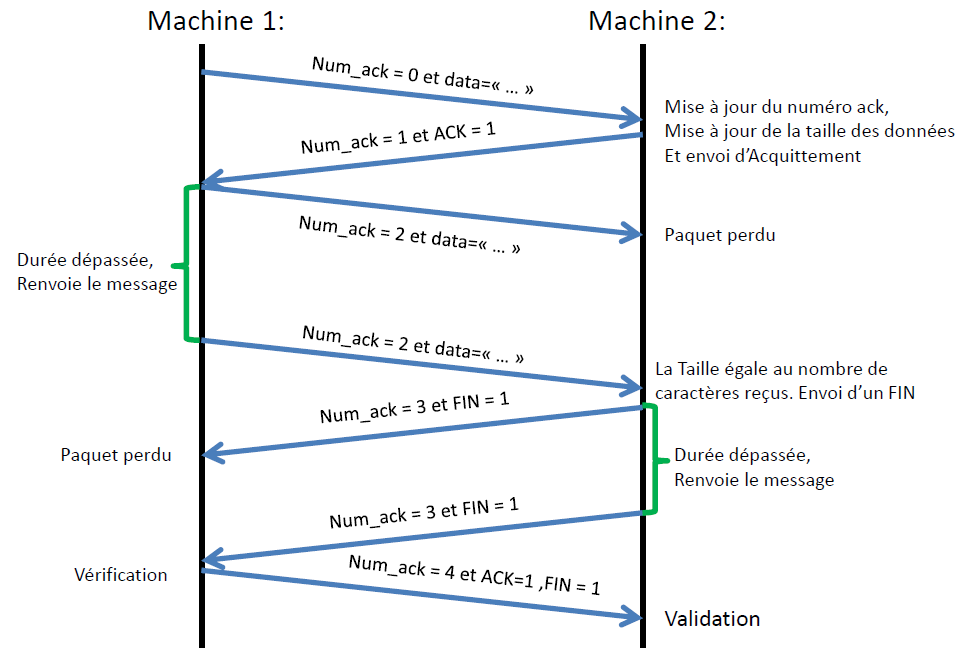
\includegraphics[scale=0.6]{protocoleReseau}
\end{center}

\bigskip


Les longs messages dépassant la taille d’une trame sont gérés par
un séquencement et l’ajout d'une taille totale dans l’en-tête de la classe MailHeader. \\


Les messages sont vérifiés grâce à leur numéro d'acquittement et par leur type ACK, FIN ou donnée, ceci dans le but de conserver l'ordre des messages et d'assurer une commmunication cohérente entre le récepteur et l'émetteur.


\chapter{Tests utilisateur}
\section{Test sur la console :}



\chapter{Organisation du travail en équipe}
Répartition des tâches



\chapter{Retour global sur le projet}

[à remplir à la fin]

\end{document}